\chapter{Introduction} % Main chapter title
\label{Chapter1} % For referencing this chapter elsewhere, use \ref{Chapter1}


\noindent 
\section{Literature review}
\noindent In medical studies, the paradigm of survival analysis is used to determine outcome events based on patient survival data. Due to the censoring complexities and high dimensionality, these datasets often entail, formal statistical approaches have been developed chronologically, each iteration improving and building upon fundamental statistical properties of survival data and the underlying result interpretation. 
\subsection{Background} 
\noindent \parencite{burzykowski_survival_2024} Reviewed the foundational concepts of survival analysis and explains it is used to examine the time until the occurrence of an event, like disease relapse. A major challenge in this area is handling censored data, where the event information is incomplete. Censoring can be of different types; right-censored data is when the event has not occurred by the end of the observation period, left-censored data is when the event occurred before the study began, and interval-censored data is when the event occurred between two observed times. To analyze such data, statistical methods have been developed.\parencite{burzykowski_survival_2024} Non-parametric methods like the Kaplan-Meier estimator and the Logrank test do not assume any specific distribution for the time-to-event data, making them robust against mis-specifications of the event-time distribution. Parametric methods like the Exponential and Weibull models assume a known distribution that models the time-to-event data. They are typically more precise, at the risk of introducing bias when the assumed distribution is wrong. \par \noindent The Proportional Hazards Model, which can be used in both semi-parametric (Cox model) and parametric forms, is employed to estimate the hazard ratio, which is a measure of effect size regarding the time to event. For instance, studies may compare the time until the onset of motion sickness under different conditions to assess treatment effectiveness. \parencite{polce_guide_2023} Explain, that traditional statistical methods require explicit programming and often suffer from user bias in variable selection, whereas Machine Learning (ML) operates under a paradigm where algorithms autonomously identify patterns in large data sets, which potentially increases accuracy and efficiency. \parencite{polce_guide_2023} Show that the literature on ML in orthopedics, predominantly composed of preliminary studies, frequently lacks depth in addressing complex ML concepts and falls short in providing comprehensive method spesification for result interpretation. \parencite{polce_guide_2023} Continues to explain that deep Learning is a prominent subset of ML, utilises neural networks to process both structured and unstructured data, enhancing the capability to handle diverse data types like images and texts. Similarly \parencite{smith_scoping_2022} show out of their methodical study selection process that only a handful of studies have attempted such comparisons at an acceptable standard, while most studies focus predominantly on machine learning techniques neglecting the broader spectrum of statistical methods. Furthermore \parencite{smith_scoping_2022} point out authors often omit interaction terms and non-linear covariate effects which are essential components for enhancing model robustness and accuracy. The predominance of studies failed to relax the proportional hazards assumption which underscores a critical oversight in adapting models to more complex datasets. Finally and more broadly \parencite{smith_scoping_2022} show that there is a need for comprehensive methodological improvements and enhanced reporting standards to ensure reproducibility and a fair assessment of method capabilities.

\begin{figure}
	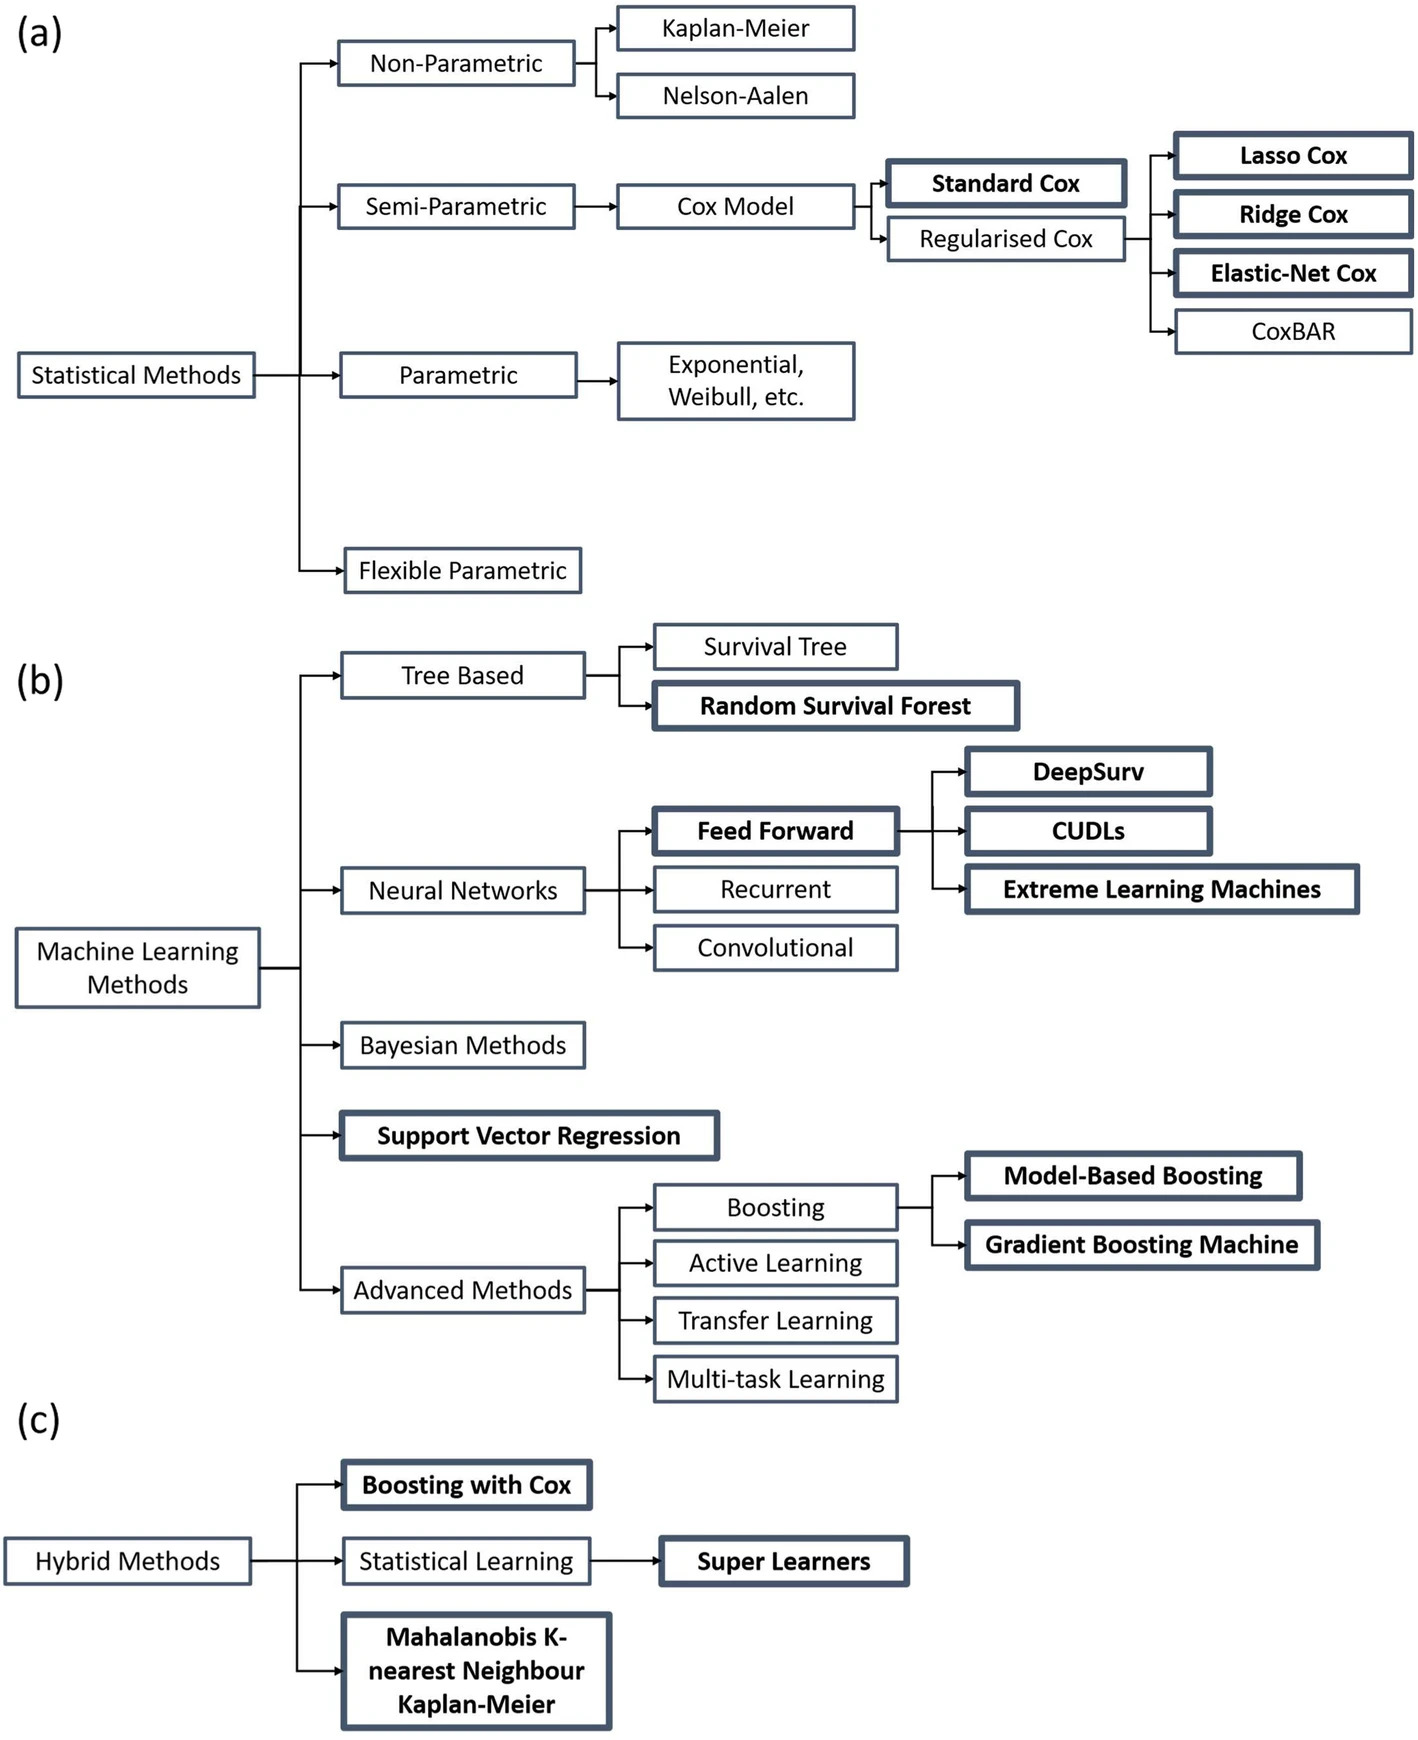
\includegraphics[scale=0.3]{Figures/ML_STATS_MODELS.jpg}
	\caption{Shows the breakdown of methods analysis preformed by \parencite{smith_scoping_2022} during a method review. The Study ran a literature selection process based on qualitative and quantitative metrics of methodology used in studies.}
\end{figure}
\subsubsection{Important issues in comparative simulation studies}

\noindent 
Simulation studies are a crucial statistical tool used for evaluating and comparing different statistical methods, particularly when analytic solutions are hard or impossible to achieve \parencite{morris_using_2019}. These studies generate data through pseudo-random sampling from known probability distributions, enabling researchers to empirically test the behavior of statistical methods under varied scenarios. Common uses include validating new statistical methods, ensuring accuracy in mathematical models and code, and comparing the effectiveness of various approaches. Particularly in medical statistics, simulation studies help in designing experiments, determining sample sizes, and estimating power under specific assumptions about data generation \parencite{morris_using_2019}. Despite their widespread use, many statisticians face challenges in properly conducting simulation studies due to a lack of understanding and experience \parencite{morris_using_2019}. Common issues include inadequate design and reporting that lead to uncritical acceptance of results. This lack of rigor can result in misleading conclusions, for example, the variability introduced by different sets of random numbers in Monte Carlo simulations that is sometimes ignored. \parencite{smith_scoping_2022} Found a notable scarcity of quality comparative research between statistical and machine learning methods. Predominantly, these studies focus on machine learning techniques while traditional statistical methods are often neglected. For instance, it was common for some authors to overlook the inclusion of interaction terms and non-linear covariate effects in the Cox model as well as time-dependent effects which are key elements for effectively handling complex datasets. The reporting standards of the reviewed studies were also generally poor. Important details such as data-generating mechanisms (DGMs), estimands, and method implementations are frequently underreported, which impedes the reproducibility of the research and the ability to conduct fair comparisons between methods. \parencite{smith_scoping_2022} Also pointed out that a significant bias could be observed in the selection of DGMs, which tend to favour machine learning approaches, especially in scenarios where the number of variables exceeds the sample size. This predisposition can lead to biassed results unless the study incorporates specific statistical variable selection techniques that are suited for high-dimensional data. Additionally, the prevalent use of the C-index as the sole performance metric, without accounting for calibration is noted. By relying solely on this metric results analysis may not provide a complete picture of the model's predictive accuracy over time, particularly when the proportional hazards assumption is not valid. Finally, \parencite{smith_scoping_2022} exclaim that there is a concerning lack of expertise in implementing complex statistical methods thoroughly. This deficiency often results in potentially misleading outcomes that do not genuinely reflect the true performance capabilities of the methods being compared. The findings underscore the need for improved methodological rigor and enhanced collaboration among researchers to ensure that both statistical and machine learning methods are implemented to their full potential and evaluated fairly. As a framework \parencite{pawel_pitfalls_2024} formalizes the use of indicators, defined as “questionable research practices” (QRP) which indicate faulty research methods used widely throughout simulation studies, which should get the necessary attention. The QRP’s are categorized during phases of comparative simulation, namely the design phase, execution phase, and reporting phase. \parencite{pawel_pitfalls_2024} Labels specific components of simulation studies, an example being D1 which references “the data-generating process”, and cross correlates with other components to define QRP occurrence and relationships.

\begin{figure}[h]
	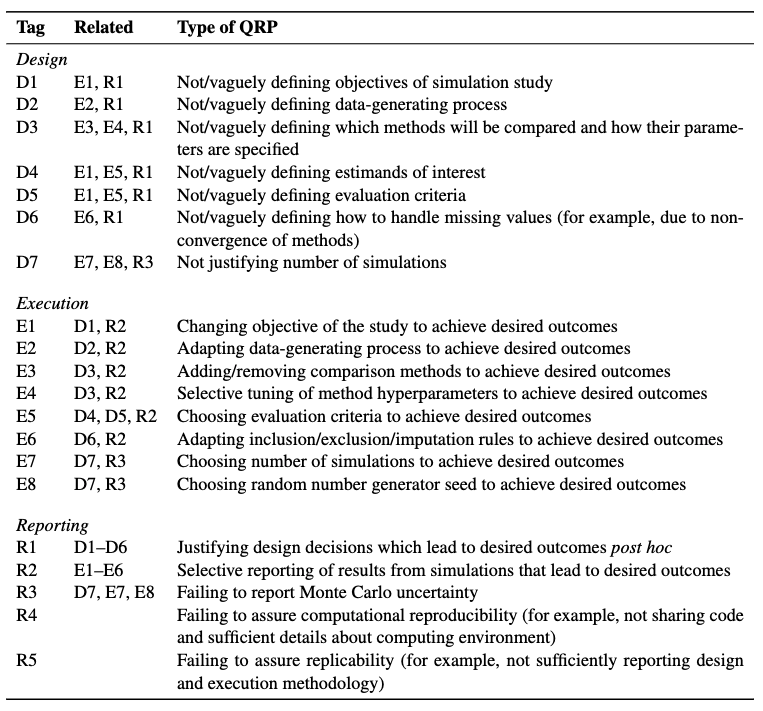
\includegraphics[scale=0.5]{Figures/QRPSUMMARY.png}
	\caption{Shows the outline of QRP classes and instances. \parencite{pawel_pitfalls_2024}}
\end{figure}

\subsubsection{Applied examples of simulation studies}

\noindent \parencite{kurt_omurlu_comparisons_2009} Evaluated and compared the effectiveness of Cox regression analysis (CRA) and random survival forests (RSF) through both simulated and actual breast cancer data scenarios. Initially, the study utilised Monte Carlo simulations to assess how both methods performed across various sample sizes, specifically observing their performance metrics based on Harrell's concordance index. The results indicated that CRA consistently outperformed RSF under simulation conditions, particularly when using the concordance index for evaluation. Following the simulations, the methods were applied to a real dataset comprising 279 breast cancer patients to identify major risk factors influencing disease-free survival (DFS). In this practical application, RSF slightly edged out other methods, offering marginally better performance according to the concordance index when using the approximate log-rank splitting rule, compared to the other log-rank rules. Approximate log-rank splitting rule:

\begin{equation} \label{eq:logrankapprox}L_{A}(X,C) = \frac{D^{1/2}(D_{1} - \sum_{t=1}^{n} I\left\{ x_{l} \le c\right\}\hat{H}(T_{l}))}{\sqrt{\left\{ \sum_{l=1}^{n} I\left\{ x_{l} \le c\right\}\hat{H}(T_{l})\right\}\left\{D-\sum_{t=1}^{n}I\left\{ x_{l} \le c\right\}\hat{H}(T_{l})\right\}}}\end{equation}

\noindent \parencite{kurt_omurlu_comparisons_2009} CRA was noted for its predictive accuracy across different sample sizes, making it suitable for a broad range of survival data applications. Conversely, RSF was recommended for its interpretative power, especially beneficial in handling complex datasets where multiple survival trees are analysed.
\\
\par \noindent Furthermore, \parencite{kantidakis_simulation_2021} shows a comparison between a machine learning method, termed survival neural networks (SNNs) and compared it with the Cox proportional hazards model, using clinical trial data for survival outcomes. The models are formulated subject to the European Osteosarcoma intergroup trial data, which is used as the foundation for the synthetic data generation that would ultimately be used for simulation training. The original dataset contains various instances of censoring, and the authors approach this issue, by segmenting the datasets into samples with degrees of censoring present (20\%, 40\%, 61\%, 80\%), afterwhich data imputation techniques such as the inverse probability weighting, censoring method (IPW), was used, which is based on calibration procedures outlined in the paper, to ensure the synthetic data retains the statistical properties of the original clinical data. The architecture used: 

\begin{equation} \label{eq:snnhazard}\lambda(x_i, \alpha_l, w) = f \left[ w_{0k}' + \sum_{h=1}^{H} w_{hk}' g_h  \left( w_{0h} + w_{1h} \alpha_l + \sum_{j=1}^{p} w_{(j+1)h} x_{ij} \right)  \right]\end{equation}

\noindent Where \(j = 1, 2, \dots , J\) are the nodes in the input layer, \(h = 1, 2, \dots , H\) are the nodes in the hidden layer, and w are the weights of the network. The training is performed with training sets and validation sets, using cross-validation and hyperparameter tuning. Furthermore, evaluation techniques are explored, specifically looking at factors like discrimination (C-index) by using the average time dependant nonlinear prognostic index,

\begin{equation} \label{eq:progindex}\theta(x_i, \alpha_l, w) = \log \left[ \frac{\lambda(x_i, \alpha_l, w)}{1 - \lambda(x_i, \alpha_l, w)} \right],\end{equation}

\noindent Accuracy (Brier) interpreted in continuous form as the integrated Brier score for prediction error over the total period,

\begin{equation} \label{eq:brier}\text{Brier}(y, \hat{S}(t_0 | x)) = (y - \hat{S}(t_0 | x))^2,\end{equation}

\begin{equation} \label{eq:briererr}\text{Err}_{\text{score}} (\hat{S}, t_0) = -\frac{1}{n} \sum_{i} \{d_i = 1\{t_i > t_0\}\} \cdot \text{score}(1\{t_i > t_0\}, \hat{S}(t_0 | x_i)) \cdot \frac{1}{\hat{C}(min(t_i - t_0) | x_i)}\end{equation}

\noindent And lastly Miscalibration (mean squared error) for censored groups. \parencite{kantidakis_simulation_2021} The results indicated comparable predictive performance but highlighted a lack of accuracy for calibration measures with SNNs. The authors point out that although machine learning techniques are attractive for survival analysis scenarios because of the ability to model interactions and nonlinearities with a no assumption approach, the robustness of the Cox model, regarding ease of implementation as well as interpretability of covariates makes it formidable in situations where limited sample sizes and variables are available. The paper ties in nicely with the other literature in support of the need for clear and better implementation of calibration metrics specifically with machine learning models, and caution against indiscriminate application of these models.


\subsection{Cox's Proportional Hazards Model}

\noindent In the seminal work by \parencite{cox_regression_1972}, the cox model is introduced as an extension to prior work formalised as the Kaplan-Meier estimator, by exploring time-to-event data (life tables). The major benefit is that it addresses censored data, which is a known concept in survival analysis, that there is missing information within the data, specifically, event occurrence without observation on a continuous time scale. The proposition consists of covariates, known as attributes regarding a unit in a distribution of data, which is associated with a coefficient \(\beta\) scaling the impact of said covariates; this product is then bound by the baseline hazard \(h_{0}(t)\).
\begin{equation} \label{eq:cox}h(t|X) = h_0(t) \exp(\beta_1 X_1 + \beta_2 X_2 + \ldots + \beta_n X_n)\end{equation}
\noindent Hazard being the estimated conditional probabilities, in line with the observed conditional frequencies of events or simply the risk of event occurrence at a specific time. An assumption of the Cox model is the proportional hazards assumption, suggesting that the hazard ratios for different covariates remain constant over time we see this for two events observations,
\begin{equation} \label{eq:coxph}\frac{h(t|X_1)}{h(t|X_2)} = \frac{h_0(t) \exp(\beta^T X_1)}{h_0(t) \exp(\beta^T X_2)} = \frac{\exp(\beta^T X_1)}{\exp(\beta^T X_2)} = \exp(\beta^T (X_1 - X_2))\end{equation}
\noindent This is an operational Assumption and a limitation as this is not always true for survival data. The model can handle censoring, by adjusting the likelihood function for observations where event occurrence did not happen in a particular continuous time frame, and by maximising the likelihood of all observed events, it is possible to estimate the coefficients that could work the best under the Cox formulation.
\begin{equation} \label{eq:coxlikely}L(\beta) = \prod_{i: \delta_i = 1} \frac{\exp(\beta^T X_i)}{\sum_{j \in R(t_i)} \exp(\beta^T X_j)}\end{equation}

\subsubsection{Time-Dependant Covariates}
\noindent The Cox model incorporates both time-independent and time-dependent covariates. \parencite{kalbfleisch_fifty_2023} Time-dependent covariates can change over the time, such as \(Z_{2}(t) = Z_{1}t^{*}\). This flexibility allows the model to handle scenarios where hazards are not proportional, which extends its applicability. Relative risk is represented as \(\exp{Z(t)'}\), showing how risk changes with time and covariate values and depending on the coefficients, the relative risk in a treatment group can increase, decrease, or remain constant over time. \parencite{kalbfleisch_fifty_2023} External covariates are variables that are independent of the subject's survival process. Whereas internal covariates are variables that might influence and be influenced by survival. \parencite{kalbfleisch_fifty_2023} Different approaches for modelling survivor functions are required for external and internal covariates due to their nature.

\noindent Proposes a step-by-step development and testing of time dependence in the Cox model, with emphasis on methods and critical formulas to highlight key concepts in understanding and applying time-dependent effects in survival analysis. \parencite{woo_time_2023} Point out how  the impact of variables can change over time, which is critical for understanding complex dynamics in data that cannot be captured by static models. Step 1 includes the selection and justification of the appropriate survival time variable for use in the Cox model. Accurate identification of the "at risk" period is crucial for defining when subjects are susceptible to the event of interest. The measurement scale (e.g., years, and months) should match the scale of independent variables. It is noted about 50\% of reviewed studies properly justified their choice of survival time variable, highlighting the need for clear explanation. Step 2 is for developing time-dependent moderation hypotheses based on a priori theory-building. It is a good indication of the importance of time dependence as it directly show effects between \parencite{woo_time_2023} the three types of time-dependent effects are type 1; both main and moderation effects are significant and in the same direction, thereby strengthening each other. Type 2; main and moderation effects are significant but in opposite directions, thereby weakening the main effect. Type 3; only the moderation effect is significant with no main effect, showing causality only in extended survival times. Step 3, tests for the proportional hazards assumption, using graphical methods like log-log survival curves. \parencite{woo_time_2023} This however is subjective and lacks statistical tests, problematic with continuous variables. Another approach is to approximate goodness-of-fit by using the Schoenfeld residuals test, which can detect non-zero slopes in survival time against scaled Schoenfeld residuals to check PH assumption violations. Step 4: Shows the extended Cox Model by integrating time-dependence detected from PH tests and adding interaction terms to the model. Interaction terms are the product of time and independent variables to handle non-proportional hazards. The extended Cox model equation:

\begin{equation} \label{eq:coxtime}h(t,X) = h_{0}(t).\exp{b_{1}x+b_{2}xt+b_{3}z}\end{equation}

\noindent Lastly Step 5 is to interpret the effects of the time dependance integration by computing hazard ratios over time to understand changes in effects due to survival time, using the extended model. \parencite{woo_time_2023} This allows the use of model results to further develop or adjust theoretical assumptions based on observed data. Hazard Ratio calculation for time-dependence, posteriori theory-building: 

\begin{equation} \label{eq:coxtimeratio}\hat{HR} = \exp{b_{1}+b_{2}t}\end{equation}

\subsubsection{Discrete vs Continuous Model}
\noindent \parencite{kalbfleisch_fifty_2023} Discrete Models address survival data that is categorical or not continuously distributed while the continuous model proposed by Cox, utilizes continuous data to model hazard functions. The survivor function can also be represented as a product integral that accommodates both discrete and continuous survival data. This approach allows for the unified handling of mixed data types in survival analysis. For the continuous model, estimation is based on maximising the conditional likelihood across observed failure times, while the discrete model uses a logistic framework for estimation, treating survival as a sequence of binary outcomes.

\subsubsection{Likelihood Function}
\noindent The various approaches to the Cox model handle data ties and time-dependent covariates differently, \parencite{kalbfleisch_fifty_2023} recommended specific methods based on the data structure (e.g., number of ties). The concept of partial likelihood is particularly important as it provides a way to focus on relevant factors in the presence of complex data types, enhancing both the theoretical understanding and practical application of the Cox model. The marginal likelihood approach \parencite{kalbfleisch_fifty_2023} (Kalbfleisch \& Prentice, 1973), was developed for both uncensored and censored data. In uncensored scenarios, it treats the ranks of data points as arising from the marginal distribution, leading to the Cox likelihood. It allows for a statistical handling of tied data points by breaking ties in all possible ways, which though accurate, is computationally intensive. \parencite{kalbfleisch_fifty_2023} Breslow's step function approach (1974), assumes a step function for the baseline hazard with changes at observed failure times. Simplifies computations but is less theoretically satisfying as the model depends on the data itself. This approach is particularly useful for handling time-dependent covariates. \parencite{kalbfleisch_fifty_2023} Bailey's non-parametric approach (1984), which uses a nonparametric maximization of the full likelihood. This provides estimators for regression coefficients and survival probabilities similar to those in previous methods. Finally the partial likelihood \parencite{kalbfleisch_fifty_2023} (Cox, 1975), uses partial likelihood for estimation, separating the effect of nuisance parameters. This approach simplifies the computational process and can isolate useful data from noise.


\subsubsection{Competing Risks}
\noindent When dealing with multiple event types, cause-specific hazard is useful for understanding mechanisms behind each cause, whereas the subdistribution hazard is useful for estimating the probability of an event occurring due to specific causes. These concepts and formulas help in modelling time-to-event data where multiple types of events can occur. In scenarios like failure time models, multiple causes might lead to an event (failure), but only the first occurring cause is observed. \parencite{kalbfleisch_fifty_2023} Shows the 'alarm clock' model proposes that each cause of failure has a separate timer, and failure occurs at the earliest timer. The Cause-Specific hazard function, is defined for each cause, representing the immediate risk of failing from that cause, given survival until time \(t\) and covariates \(Z\).
\begin{equation} \label{eq:spesifichazard}h_{j}(t|Z) = \lim_{h \to 0} \frac{P(t \le T < t+h, J=j|T\ge,Z)}{h} \text{for} j=1,\dots,m\end{equation}

\noindent The survivor function used calculates the probability of surviving (not failing) past time \(t\) considering all causes.

\begin{equation} \label{eq:spesificsurvivor}S(t|Z) = \exp(-\int_{0}^{t} h(u|Z) du)\end{equation}

\noindent Cumulative Incidence Function is shown to be the probability of failing from cause \(j\) by time \(t\), accounting for competing risks.

\begin{equation} \label{eq:cumulativeincidence}F_{j}(t|Z) = \int_{0}^{t} h_{j}(u|Z)S(u|Z)du\end{equation}

\noindent The subdistribution hazard \parencite{kalbfleisch_fifty_2023}(Fine \& Gray Model), specifically focuses on the hazard of a particular cause while considering other causes as competing events, by directly modelling the cumulative probability of the event of interest.

\begin{equation} \label{eq:subdistribution}\tilde{a}_{j}(t|Z) = \frac{d}{dt}log(1-F_{j}(t|Z))\end{equation}

\subsection{Lasso Regularisation And Variable Selection}
\noindent The Lasso technique \parencite{tibshirani_regression_1996}, a regression analysis method introduced to address specific limitations of Ordinary Least Squares (OLS) estimation, is particularly beneficial in scenarios with a large number of predictors or high collinearity among them which would mean that models could produce inflated variance scores, and cause impaired interpretability. Lasso optimises prediction accuracy and enhances model interpretability by employing a shrinkage process that can set certain coefficients to zero effectively, thus performing variable selection.

\begin{equation} \label{eq:lasso}\hat{\beta}^{lasso} = \arg \min_{\beta} \left\{ \frac{1}{2N} \sum_{i=1}^{N} (y_i - \beta_0 - \sum_{j=1}^{p} X_{ij}\beta_j)^2 \right\}\end{equation}

bound by,

\begin{equation} \label{eq:lassobound}\sum_{j=1}^{p} |\beta_j| \leq t.\end{equation}

\noindent \parencite{freijeirogonzalez_critical_2022} The inclusion of the regularisation term, is crucial as it allows for the reduction of model complexity by penalising the magnitude of the coefficients, which promotes sparser models. This sparsity is instrumental in enhancing interpretability by isolating only the most significant predictors that contribute to the dependent variable. The objective function of LASSO is convex for \(l_{1}\) norm, which simplifies finding the global minimum. Multiple optimal solutions might exist, especially when the number of predictors \(p\) exceeds the number of observations \(n\). \parencite{freijeirogonzalez_critical_2022} LASSO introduces bias in the coefficients to achieve lower variance and better model parsimony. Consistent under conditions like the irrepresentable condition, crucial for variable selection. Bias Correction achieved via,

\begin{equation} \label{eq:lassobais}\hat{\beta}_{j}^{LASSO}=sign(\hat{\beta}_{j}^{OLS})(|\hat{\beta}_{j}^{OLS}| - \lambda)_{+}\end{equation}

\noindent By penalising the sum of the absolute values of the model parameters, the LASSO method encourages models with fewer parameters. This can lead to the exclusion of some variables entirely if their effect is not strong enough to justify a larger coefficient size given the regularisation penalty. LASSO can incorrectly include or exclude important variables, known as false discoveries. Enhanced methods like Adaptive LASSO, Stability Selection are used to improve variable selection accuracy. The choice of \(\lambda\) affects the sparsity of the resulting model; too large a \(\lambda\) might shrink all coefficients to zero. The \(\lambda\) parameter is often chosen via cross-validation by optimising some criterion (e.g., AIC, BIC, MSE). \parencite{freijeirogonzalez_critical_2022}Popular extensions of the lasso method include:

\begin{tabularx}{\textwidth}{|X|X|X|}
	\hline
	Method & Library & Description \\
	\hline
	LASSO & glmnet & Regularized regression that encourage sparse solutions by adding a penalty proporional to the absolute value of the coefficients. \\
	\hline
	SCAD & ncvreg & Non-convex penalty that encourages sparsity without overly penalizing large coefficients, more continuity in coefficient estimation compared to Lasso \\
	\hline
	Adaptive Lasso & adapl \& glmnet & weights penalties based on initial estimates to improve consistency. \\
	\hline
	Dantzig Selector & Dant \& flare & Ensures residuals are small and the solution is sparse, focussing on covariate selection accuracy \\
	\hline
	Relaxed Lasso & relaxl \& relaxo & Combines Lasso solution with unpenalized least squares, reducing bias and variability  \\
	\hline
	Square-root Lasso & sqrtl \& flare & Modification of lasso stabilizing noise level variability \\
	\hline
	Scaled Lasso & Scail \& scalreg & Adjusts the penalty term dynamically based on residual variance, improving error rate and variable selection \\
	\hline
\end{tabularx}
\subsubsection{Adaptive Lasso}
\noindent By using weights that are inversely proportional to the magnitude of initial estimates, \parencite{zhang_adaptive_2007} Adaptive Lasso can differentiate more effectively between relevant and irrelevant predictors, for variable selection. Regularisation helps prevent overfitting, a common issue in models trained on high-dimensional data. \parencite{zhang_adaptive_2007} By penalizing the sum of the absolute values of the coefficients, the Adaptive Lasso ensures that the model generalizes well to unseen data. Compared to the standard Lasso, the adaptive version reduces the bias in the estimation of large coefficients, which is beneficial when true model coefficients vary in size. The log partial likelihood for the Cox model, as given by:

\begin{equation} \label{eq:likelihood}l(\beta) = \sum_{i:\delta_{i}=1} \left[ \beta^{T}x_{i} - \log{\sum_{j:t_{j}\ge t_{i}} \exp(\beta^{T}x_{j})} \right]\end{equation}

\noindent Which provides a measure of how well the model's predicted hazards match the observed data. Here, \(\delta\) indicates whether an event (e.g., failure, death) was observed at time \(t_{i}\). To minimise the Adaptive Lasso's penalised version of this likelihood:

\begin{equation} \label{eq:adaptlasso}
\text{min}\left[ -\ell(\beta) + \lambda \sum_{j=1}^{p} \frac{|\beta_j|}{|\beta_j|^\gamma} \right]
\end{equation}

\noindent The Adaptive Lasso adds a penalty that adjusts according to the initial estimates of the coefficients. This penalization mechanism performs two critical roles \parencite{zhang_adaptive_2007}, Shrinkage; coefficients estimated to be small by the initial model are shrunk towards zero more aggressively, reducing the model's complexity and enhancing interpretability, Selection; larger coefficients (i.e., those considered more significant in the initial model) are penalised less, allowing them to stand out in the final model, thus maintaining their impact on the model's predictions. Each coefficient is updated in turn, optimizing the objective function concerning one \(\beta\) while keeping the others fixed \parencite{zhang_adaptive_2007}. The algorithm iterates over all coefficients repeatedly until convergence is achieved, usually defined by a small change in the value of the objective function

\subsubsection{Outcome Adaptive Lasso}
\noindent The Outcome-adaptive Lasso (OALasso) \parencite{shortreed_outcome-adaptive_2017} modifies the standard Lasso penalty by weighting the regularisation of each coefficient according to its association with the outcome variable. This is intended to handle situations common in causal inference where the goal is not just prediction but understanding which variables causally affect the outcome. The OALasso minimization \parencite{shortreed_outcome-adaptive_2017} problem is formulated as:

\begin{equation} \label{eq:oalasso}\underset{\beta}{\text{min}} \left\{ \frac{1}{2n} \sum_{i=1}^{n}(y_{i}-x_{i}^{T}\beta)^{2} + \lambda \sum_{j=1}^{p}w_{j}|\beta_{j}|\right\}\end{equation}

\noindent Where \(w_{j}\) are weights that are inversely proportional to the absolute values of the estimated coefficients from a preliminary unpenalized regression on the outcome. This weighting scheme is calculated as follows:

\begin{equation} \label{eq:oalssobound}W_{j} = \frac{1}{|\hat{\beta}_{j}^{OLS}|^{\gamma}}\end{equation}

\noindent The term \(\hat{\beta}_{j}^{OLS}\) is the ordinary least squares estimates for each predictor. \(\gamma\) is a tuning parameter that determines how the weights decay; commonly set to values like 0.5 or 1 depending on the desired sensitivity. The penalty weights \(w_{j}\) ensure that predictors with smaller absolute coefficients in a simple OLS regression on the outcome are penalised more heavily, under the assumption that they are less likely to be causally related to the outcome. By focusing the regularisation in this way, \parencite{shortreed_outcome-adaptive_2017} OALasso aims to retain variables in the model that are more likely to be true causal factors rather than merely correlated with the outcome. The outcome-adaptive weighting mechanism can be justified theoretically by considering the bias-variance tradeoff and the properties of estimators in high-dimensional settings. Predictors with large coefficients are less likely to be due to random fluctuations in the data; hence, reducing their penalty helps to reduce bias without a substantial increase in variance. The \(\lambda\) and \(\gamma\) parameters must be carefully tuned, often via cross-validation, to balance the complexity of the model against the risk of overfitting. This method is more computationally intensive than standard Lasso due to the need for preliminary OLS estimation and weight calculation, OALasso can be implemented efficiently using iterative algorithms \parencite{shortreed_outcome-adaptive_2017} similar to those used for other Lasso variations.


\subsection{Random Surivival Forest}
\noindent Random survival forests \parencite{ishwaran_random_2008} are an extension of random forests, which have the ability to handle right-censored data and aim to estimate the appropriate survival function. Consisting of an ensemble of trees \parencite{ishwaran_random_2008}, which are grown from a bootstrap sample, and each node of underlying trees, consists of specific covariates due to a random selection of features for splits in each tree. Random forests are adapted for survival analysis by modifying how predictions are aggregated to handle censored data effectively. Forest survival function estimator:
\begin{equation} \label{eq:rsfestimator}\hat{\Lambda}(t, x_{0}) = \frac{1}{B} \sum_{b=1}^{B} \hat{\Lambda}_{b}(t,x_{0})\end{equation}
Survival function:
\begin{equation} \label{eq:survrsf}S(t,x_{0}) = \exp^{-\hat{\Lambda}(t,x_{0})}\end{equation}

\noindent To reduce tree correlation and prevent overfitting \parencite{pham_springer_2023}, two main mechanisms are used namely bagging (Bootstrap Aggregating) and random feature selection at each split. Tuning common parameters like the number of trees (ntrees), the number of features (mtry) considered at each split, and the minimum sample size per node (nmin), is critical for optimising random forest performance. A benefit of the model is within its ability to capture survival functions for an individual in the distribution by estimating its survival function across all trees where the individual is captured in terminal nodes. Per node splitting criteria are conditional to survival time and censoring, whereby node “impurity” \parencite{ishwaran_random_2008} is determined by the survival differences. Methods like log-rank, conservation of events splitting rule, and random log rank are used. Terminal nodes are the result of saturated splitting criteria, with each endpoint having d-dimensional covariates of the individuals encapsulated. A key component of the model is the conservation of events principle, which is used to define a type of predicted outcome, namely ensemble mortality, which is derived from the cumulative hazard function (CHF) using the Nelson-Aalen estimator in the original paper by \parencite{ishwaran_random_2008}. Terminal nodes or nodes at the end of tree branches all share the estimated hazard function. Another key concept is the out-of-bag (OOB) samples which act as a validation subset \parencite{ishwaran_random_2008}. The OOB error is calculated on the ensemble survival function with regard to the observed data using metrics like concordance (C-index). Used for estimating prediction error and model performance without a separate test data set. Each tree's error is calculated using data not included in its training set (out-of-bag). Prediction error metrics, like the concordance index which calculates the permissible pairs per node and OOB prediction error, are used for accuracy metrics. 

\begin{equation} \label{eq:ooberror}
\hat{\Lambda}_{oob}(t,x_{i}) = \frac{1}{\sum_{b=1}^{B}I(x_{i}\in L^{b}_{oob})}\sum_{b=1}^{B}I(x_{i}\in L^{b}_{oob})\hat{\Lambda}_{b}(t,x_{i})
\end{equation}

\noindent It is important to note here that \parencite{ishwaran_random_2008} puts forward an approach to deal with missing data, outlining the short-comings of prior methods like replacing missing values with distribution medians, and for categorical data replacing with most frequent occurrences. The method is called adaptive tree imputation and relies on the OOB data set to determine missing data, for both continuous or integer values. This method is a part of the model and deals with censoring implicitly, which is different from external simulation and imputation methods. Variable importance (VI) \parencite{pham_springer_2023} in random forests is used to rank variables based on their contribution to prediction accuracy. It is assessed by looking at each predictor variable in the sample and assessing the impact on prediction error, an increase in error indicating importance. Different random forest settings can yield different importance rankings due to the model's sensitivity to the configuration. VI is shown by \parencite{pham_springer_2023}:
\begin{equation} \label{eq:vinorm}
VI(j) = \frac{1}{B}\sum_{b=1}^{B}(\frac{Err(j)_{b}}{Err_{b}}-1)
\end{equation}
\noindent A benefit of the model is well suited for high dimensional data because of the random subset selection process, which helps mitigate overfitting. Due to the permutative nature of the ensemble bound to the brevity of the underlying data distribution, the model is computationally demanding \parencite{pham_springer_2023}, and although the model can yield variable information, it might be difficult to interpret the final resulting model, because the correlated variables doesn't necessarily account for mutual information between.

\begin{equation} \label{eq:viadapt}VI(j) = \frac{1}{B}\sum_{b=1}^{B}(\frac{Err(j|Z)_{b}}{Err_{b}}-1)\end{equation}

\noindent This adaptation \ref{eq:viadapt} addresses correlations \parencite{pham_springer_2023} by conditioning on other related variables. This accounts for the influence of correlated predictors by adjusting the variable importance calculation.

\subsubsection{Relative Risk And Conditional Inference Extensions}
\noindent \parencite{yao_ensemble_2022} points out that the counting process approach is used to handle time-varying covariates by assuming that these covariates are constant between observed time points. Each subject's observations are split into multiple "pseudo-subjects" based on the intervals between these time points. Each pseudo-subject is treated as an independent observation with specific covariate values constant over the interval from one observation to the next. This provides a framework to accommodate right-censoring and left-truncation. \parencite{yao_ensemble_2022} Extends both forest algorithms, conditional inference forest (CIF-TV) and relative risk forest (RRF-TV) to include time-varying covariates. In CIF-TV, recursive partitioning is performed by testing the independence of survival times from covariates within each node of the tree using modified log-rank scores that consider censoring. In RRF-TV, the partitioning criterion maximises the reduction in deviance, reflecting better fit between observed and modelled survival times at each tree node. The modified log-rank scores and the new deviance reduction criteria is adapted for time-varying covariates to provide a more nuanced analysis of the data. \parencite{yao_ensemble_2022} show two bootstrapping options for out-of-bag splits, bootstrapping subjects by keeping all pseudo-subjects for each subject together and bootstrapping pseudo-subjects by treating each pseudo-subject as an independent observation. Several parameters, such as the number of variables considered at each split (mtry), the minimum size of terminal nodes, and others, are tuned to optimise the model performance. These parameters are adjusted based on out-of-bag error estimation \parencite{yao_ensemble_2022}, which helps in selecting the best model settings without requiring a separate validation dataset. Tuning these parameters specifically for time-varying data helps in improving the precision and accuracy of the survival estimates. The use of out-of-bag samples for tuning allows for continuous improvement and validation of the model throughout the training process.

\subsubsection{Oblique Random Survival Forests}
\noindent \parencite{jaeger_accelerated_2022} shows advancements in the Random Survival Forest (RSF) algorithm, particularly through the use of oblique decision trees as opposed to traditional “axis-based”: trees. \parencite{jaeger_accelerated_2022} Axis-based trees split data using a single predictor, leading to decision boundaries aligned with axes of the predictor space. Oblique trees use a linear combination of predictors for splitting, resulting in more complex, non-aligned decision boundaries. This approach can handle correlated predictors better and has been shown to improve prediction accuracy and reduce concordance error in survival analysis \parencite{jaeger_accelerated_2022}. Despite their advantages, oblique trees are computationally expensive as they might require exponentially more calculations than axis-based trees. This is mainly because evaluating potential splits in oblique trees involves considering numerous combinations of predictors. Traditional methods of assessing Variable Importance \parencite{pham_springer_2023} like permutation, are less effective for oblique trees since changing one predictor's value does not significantly impact decisions made on linear combinations of predictors. Negation Variable Importance (Negation VI) \parencite{jaeger_accelerated_2022}, a new method for assessing VIMP that involves negating the coefficients of predictors to determine the impact on prediction accuracy. This method is shown to be non-random, reproducible, and effective even when predictors are correlated. To accommodate the high computational demand, \parencite{jaeger_accelerated_2022} proposes using fast algorithms like the Newton-Raphson scoring on Cox regression models to quickly identify optimal predictor combinations in non-leaf nodes, which reduces the time and computation required for model training. The improvements and new techniques are incorporated into the 'aorsf' R package \parencite{jaeger_accelerated_2022}, which offers tools for building accelerated and interpretable oblique RSFs. Oblique trees were found to significantly enhance prediction accuracy compared to axis-based trees. Studies showed improvements in concordance error between 2.5\% to 24.9\%, depending on the dataset used.

\begin{figure}
	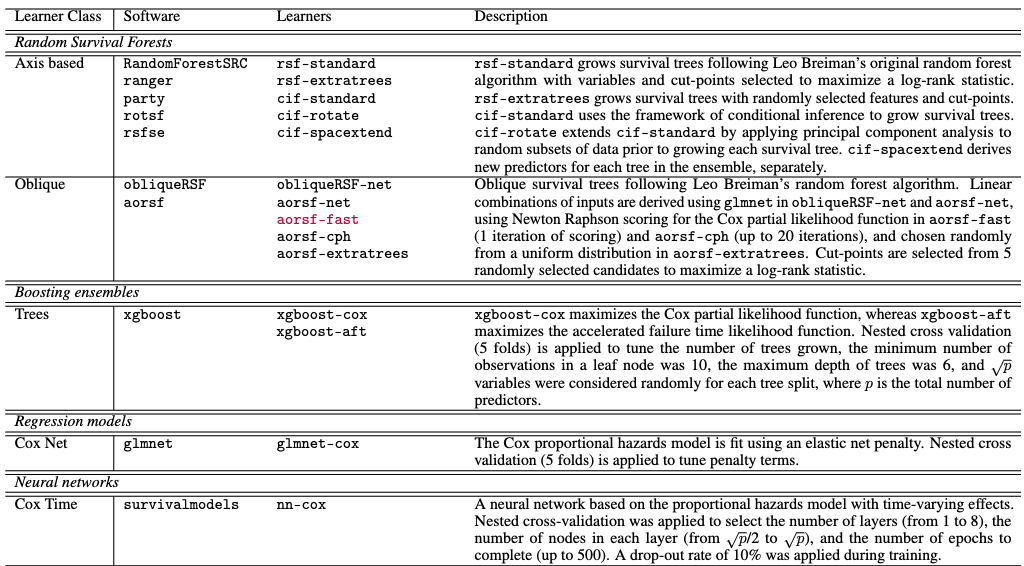
\includegraphics[scale=0.42]{Figures/OBLIQUE_SUMMARY.png}
	\caption{\parencite{jaeger_accelerated_2022} Shows available packages based on model types for random survival forests.}
\end{figure}

\subsection{Methods For Data Generating Mechanisms For Simulation}
\noindent Methods for extrapolating missing data, speaks to the key feature of survival analysis and the difficult problem of dealing with censored data. Several different methodologies and considerations exist outlining how to impute, simulate and generate data, for different settings of survival data.
\subsubsection{Data Imputation Methods}
Data imputation is crucial for addressing issues arising from censored data by replacing missing values with values that resembles others in the distribution. Censoring can occur due to various reasons such as; the end of the follow-up period, loss to follow-up, or discontinuation of study participation. This often prevents the collection of complete data on the time until an event of interest occurs and so \parencite{jin_imputation_2024} classifies censoring classes as, censored at random (CAR) and censored not at random (CNAR). Data imputation is relevant to these contexts to correct for the potential biases introduced by censoring, especially when it is informative or non-random. \parencite{jin_imputation_2024} Shows the Cox Proportional Hazards model assumes noninformative censoring (CAR) for its analysis. In cases where this assumption might not hold due to practical reasons, such as decisions influenced by patient or physician preferences, they point to data imputation under CNAR assumptions as a way to account for potential biases. Under the CAR assumption \parencite{jin_imputation_2024}, the hazard function after censoring is assumed to be the same as if the subject had not been censored, conditional on the covariates. This reflects the assumption that the censoring is non-informative regarding the survival probability. Hazard post CAR: 
\begin{equation} \label{eq:carassmp}\lambda_{post}(t|Z_{i},X_{i}(t)) = \lambda_{0}(t)\exp^{\beta Z_{i} + \alpha X_{i}(t)}, t>C_{i}\end{equation}
\noindent This means that the survival and hazard functions do not need special adjustments beyond the point of censoring other than ensuring that the analysis correctly accounts for the time of censoring. For CNAR, \parencite{jin_imputation_2024} the assumption is that the hazard of having an event after censoring may differ from that before censoring due to the censoring being potentially dependent on unobserved variables affecting the hazard. Mathematically, this means the post-censoring hazard function cannot simply extend the pre-censoring model. Hazard post CNAR:
\begin{equation} \label{eq:cnarassmp}\lambda_{post}(t|Z_{i},X_{i}(t)) \neq \lambda_{0}(t)\exp^{\beta Z_{i} + \alpha X_{i}(t)}, t>C_{i}\end{equation}
\noindent In practical terms, the CNAR model needs to be specifically formulated to reflect how the hazard might increase or decrease post-censoring due to factors related to why the censoring occurred. This could involve modifying the functional form of \(\lambda_{post}\) or using additional data and techniques to estimate it. \parencite{jin_imputation_2024} Shows 4 methods for handling data imputation under the CNAR and CAR assumptions.
\\\\
\textit{Delta-adjusted Method}
\begin{equation} \label{eq:deltaadjust}\lambda_{post}(t|Z_{i},X_{i}(t)) = \lambda_{\emptyset}(t|Z_{i},X_{i}(t)) = \lambda_{0}(t)\exp^{(1-\emptyset)\beta Z_{i} + \alpha X_{i}(t)}, t>C_{i}\end{equation}
\noindent The sensitivity parameter (\(\emptyset\)) represents a discounted proportion of the log-hazard ration \(\beta\) under the CNAR assumption. The method assumes that the hazard of having an event for censored subjects is multiplicatively decreased by a factor depending on the \(\emptyset\). The term \((1- \emptyset)\beta\) suggests a reduced effect of the treatment on the hazard rate post-censoring.
\\\\
\textit{Tipping point Analysis}
\par \noindent This method is used to identify how much the assumption of noninformative censoring (CAR) would need to be violated for the study results to become statistically nonsignificant. It uses the delta-adjusted method's parameter \(\emptyset\) to calculate the minimum shift in \(\beta\) (log HR) needed to nullify the treatment effect.
\\\\
\textit{Jump to Reference}
\begin{equation} \label{eq:jtor}\lambda_{post}(t|Z_{i},X_{i}(t)) = \lambda_{J2R}(t|Z_{i},X_{i}(t)) = \lambda_{ref}(t|X_{i}(t)) = \lambda_{0}(t)\exp^{\alpha X_{i}(t)}, t>C_{i}\end{equation}
\noindent This Method assumes that once censored, the hazard rate for a subject from the treatment group immediatly aligns with that of the reference group, completely disregarding any risidual effects of the treatment past the point of censoring.
\\\\
\textit{Copy Reference}
\begin{equation} \label{eq:copyref}\lambda_{CR}(t|Z_{i} = 1,X_{i}(t)) = \lambda(t|Z_{i} = 0, X_{i}(t)) = \lambda_{0}(t)\exp^{\alpha X_{i}(t)} \text{for all}, t\end{equation}
\noindent This method is conservative but less so than J2R in that it assumes that if a subject in the treatment group is censored, their hazard function matches that of the reference group for the remainder of the study. It does not account for any time-specific variations in hazard that might have been influenced by the treatment before censoring.
\\\\
\textit{Censored at Random}
\par \noindent Assumes noninformative censoring where the post-censoring hazard (\(\lambda_{post}\)) is identical to the pre-censoring hazard, simplifying the imputation process.

\subsubsection{Data Simulation Methods}
\noindent \parencite{thurow_how_2023} Shows that there is a scarcity of publicly available real-world datasets for benchmarking models in oncology, particularly those that comply with the FAIR Data Principles. This significantly limits the ability to conduct model comparisons using real patient data, which is crucial for ensuring the models' applicability and robustness in real-world scenarios. The challenge of simulating realistic survival data for model comparison in situations where real-world data is not available or is incomplete. This is particularly relevant for ensuring that simulated data can reliably mimic real-world outcomes to validate model performance effectively. \parencite{thurow_how_2023} proposes several methods for dealing with data simulation.
\begin{figure}
	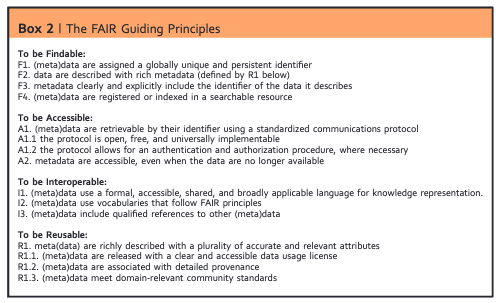
\includegraphics[scale=0.85]{Figures/FAIR_PRINCIPLES.png}
	\caption{\parencite{wilkinson_fair_2016} Fair principles summary}
\end{figure}
\\\\
\textit{Parametric Distribution}
\par \noindent This method is used to simulate survival times using predefined parametric distributions. The fit of each distribution to the data is tested using the one-sample Cramér-von Mises (CVM) test. The distribution that shows the least deviation from the data (highest p-value in the CVM test) is chosen for simulation. Parameters for these distributions are estimated using Maximum Likelihood Estimation (MLE). An Example for mixed distribution: 
\begin{equation} \label{eq:paramdist}f(x)=0.2.f_{Weibull}(\alpha,\lambda)+0.8.f_{norm}(\mu,\sigma)(x)\end{equation}
\noindent Where \(f_{Weibull(\alpha, \lambda)}\) and \(f_{norm}(\mu,\sigma)\) are the density functions for the Weibull and normal distributions, respectively.
\\\\
\textit{Kernel Density Estimation (KDE)}
\par \noindent Used to estimate by utilizing the density function of the data for simulation. The density function is estimated using the kdensity function from the \parencite{thurow_how_2023} R-package, which employs a Gaussian kernel. The Accept-reject method is used to generate random values that follow the estimated density function. Draw \((X, U)\) from the joint distribution \((X, U) ~ \left\{ (x,u):0<u<f(x)\right\}\) where X is a random variable following the estimated density f, and U is uniformly distributed between 0 and \(f(x)\). If \(u_{i} < f(x_{i})\) for a sampled \((X,U),x_{i}\) is accepted as a realization from the density function \(f\)
\\\\
\textit{Case Resampling}
\par \noindent Simulate data by resampling observed data points with replacement. Directly resample observations (ti, di) from the existing dataset of observed times and censoring indicators. \((t_{i}, d_{i})^{*}\) are drawn with replacement from \(\left\{ (t_{1}, d_{1}) \dots (t_{n}, d_{n})\right\}\)
\\\\
\textit{Conditional Bootstrapping}
\par \noindent To simulate data using bootstrapping that accounts for censoring, this helps sample censor times. For censored observations, censoring times are carried over to the simulated data. For uncensored observations, new censoring times are sampled based on the conditional distribution of censoring times given they are greater than the observed event time. Censoring Time for censored data: \(c_{i}^{*} = t_{i}\) for censored observation. Censoring Time for uncensored data: \(c_{i}^{*}\) is sampled from \(G_{i}(c) = \frac{G(c)-G(t_{i})}{1-G(t_{i})}\) where \(G\) is the distribution function of censoring times and \(t_{i}\) is the observed event time. Event times \(t^{*}_{oi}\) are sampled from the observed event times with replacement. \parencite{thurow_how_2023} show that for reconstruction of reliable benchmark data sets are meticulously reconstructed from published Kaplan-Meier plots and other vital statistics like hazard ratios and p-values from logrank tests. The data sets, particularly those with non-crossing survival curves, demonstrate high fidelity to the original data, proving them to be excellent resources for subsequent model evaluations.

\subsubsection{Simulation for competing risks and clustering}
Competing risks occur when an individual or unit under study can experience one of several different types of events, and the occurrence of one event prevents the occurrence of another. For example, in medical research, a patient might die from cancer or heart disease, and death from either cause prevents death from the other (competing) cause. These situations require specialised models, such as the Fine and Gray model \parencite{meng_simulating_2023} for subdistribution hazards, which handle the fact that the risk of the event of interest is "competed away" \parencite{meng_simulating_2023} by the risks of other types of events. These models keep individuals in the risk set even if a competing event occurs and provide insights into the probability of the event of interest in the presence of other risks. Clustering in survival data refers to situations where there are groups or clusters of observations that share a common characteristic or environment, which might affect their event outcomes. This could be because individuals are grouped naturally (e.g., families, hospitals, schools) or through the design of the study (e.g., cluster randomized trials). Individuals within the same cluster tend to have more similar event outcomes than individuals from different clusters. In this case the intra-cluster correlation must be accounted for in the analysis because standard survival models that assume independence between observations can lead to biassed or incorrect estimates.
\begin{figure}[h]
	\centering
	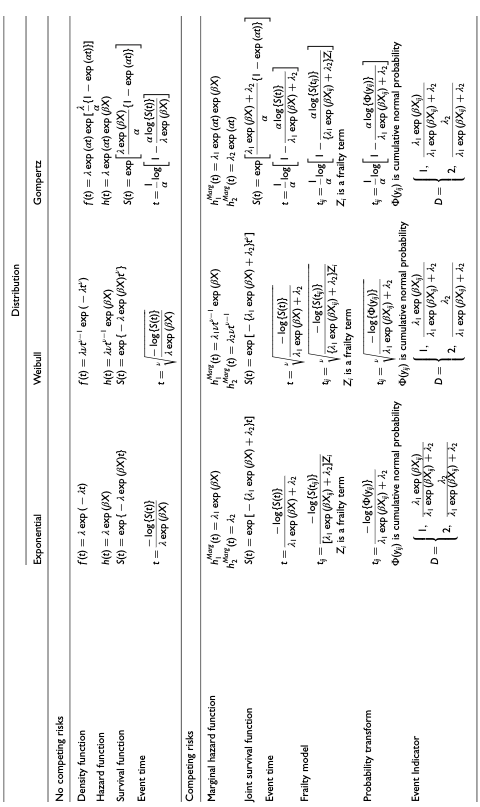
\includegraphics[scale=0.56 , angle=270]{Figures/COMPETING1.png}
	\caption{\parencite{meng_simulating_2023} shows simulation formulas under spesific conditions}
\end{figure}

\begin{figure}[h]
	\centering
	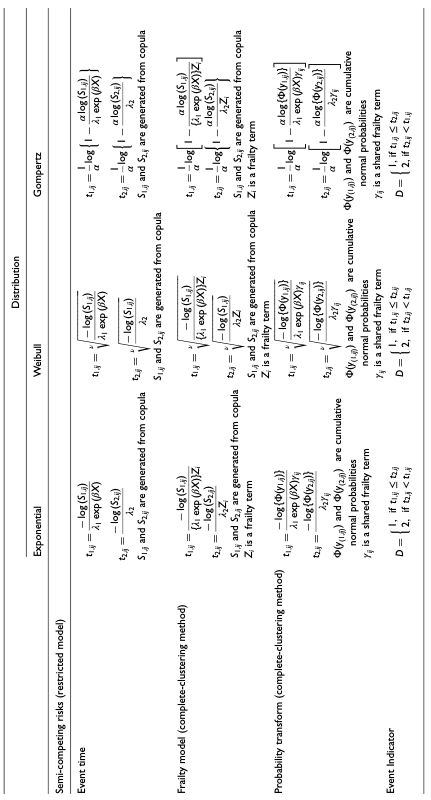
\includegraphics[scale=0.56, angle=270]{Figures/COMPETING2.png}
	\caption{\parencite{meng_simulating_2023} shows simulation formulas under spesific conditions (continued)}
\end{figure}
\subsubsection{Synthetic Data Generation Methods}
Machine learning methods for simulation and data generationhave risen in popularity recently, \parencite{norcliffe_survivalgan_2023} shows multiple methods combining statistical imputation methods into machine learning architectures. Specifically \parencite{norcliffe_survivalgan_2023} extend prior work for survival analysis to generate synthetic data using a Conditional Generative Adversarial Network (GAN) framework. The process integrates various components to handle different data types and ensure realistic simulation of survival times based on censoring and event data. Input Handling, A condition vector C and an event indicator E are provided by the user. C is a one-hot vector including interpretable features and latent encodings. E indicates whether the data point is censored (0) or an actual event (1). These inputs can either be sampled based on existing data distributions or manually selected by the user. The conditional GAN consists of a generator and discriminator trained to produce the covariate x given C and E (x ~ p(x|C, E)). The tabular encoder converts continuous features into a format suitable for the GAN using a Gaussian Mixture Model (GMM)\parencite{norcliffe_survivalgan_2023}; each feature is represented by its GMM component and deviation from the component mean. Categorical features are directly converted into one-hot vectors. The Encoder simplifies the full tabular encoding to just the one-hot vector component, representing condition C for the generator. The Survival Function is the statistical representation that outputs survival probabilities at various time points for given covariates (x). For the Survival GAN architecture, they used models like DeepHit \parencite{norcliffe_survivalgan_2023} to estimate probabilities. The Time Regressor component predicts the actual time of an event or censoring based on the outputs of the survival function and the event type (E). This component can utilise various regression models, such as XGBoost \parencite{norcliffe_survivalgan_2023}. During training the loss function used was a Wasserstein GAN \parencite{norcliffe_survivalgan_2023} with a gradient penalty which ensures stable training of the GAN by adjusting the generator and discriminator losses to minimise the distance between real and generated data distributions while penalizing gradient norms. This allows for user-defined or sampled conditions and events. The GAN uses these to generate encoded covariates, which are then decoded back to their original form. These covariates are input into the survival function and time regressor to finally produce the synthetic time-to-event data. This architecture allows SurvivalGAN to realistically model survival data by accurately simulating the underlying time-to-event dynamics and handling various data imbalances and types.

\begin{figure}
	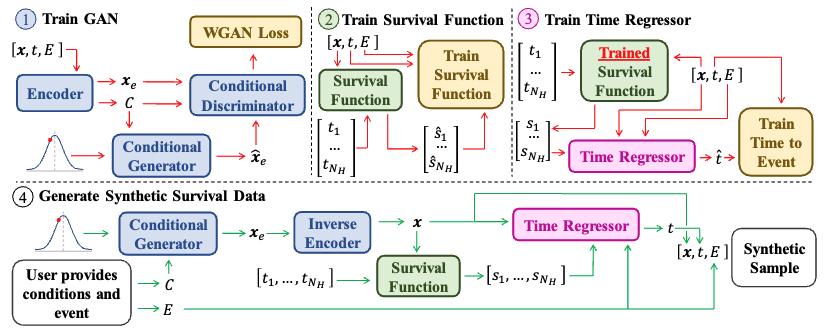
\includegraphics[scale=0.51]{Figures/GAN_ARCH.png}
	\caption{\parencite{norcliffe_survivalgan_2023} Survival GAN architecture}
\end{figure}

\noindent \parencite{norcliffe_survivalgan_2023} Employ several metrics to assess synthetic survival data according to the real dataset. They help identify and correct biases in synthetic data to better align with real-world data, enhancing the credibility of survival analysis models. The optimism metric assesses whether the synthetic data is over-optimistic or over-pessimistic compared to real data by comparing the expected lifetimes derived from Kaplan-Meier (KM) plots.
\begin{equation} \label{eq:optimisim}\text{Optimism} = \frac{1}{T} \int_{0}^{T}(S_{Syn}(t)-S_{Real}(t))dt\end{equation}
\noindent Where \(S_{Syn}(t) and S_{Real}(t)\) are the synthetic and real Kaplan-Meier survival functions respectively, and T is the latest time point available. The optimism metric ranges between -1 and 1, where values closer to 0 indicate accurate lifetime predictions, positive values suggest over-optimism, and negative values indicate over-pessimism. The short-sightedness metric quantifies how much earlier synthetic data, discontinues providing predictions compared to real data, reflecting potential censorship in the synthetic modeling.
\begin{equation} \label{eq:ssmetric}\text{Short-Sightedness} = \frac{T_{Real}-T_{Syn}}{T_{Real}}\end{equation}
\noindent Here, \(T_{Syn} and T_{Real}\) are the end times of the synthetic and real Kaplan-Meier plots, respectively. This metric ranges from 0 to 1, where 0 indicates no censorship issues and 1 indicates complete short-sightedness in the synthetic data predictions. Lastly, the Kaplan-Meier divergence measures the overall divergence between the synthetic and real KM curves across the observed time period, providing a comprehensive measure of similarity between the two datasets.
\begin{equation} \label{eq:kmdiverge}\text{KM Divergence} = \frac{1}{T}\int_{0}^{T}|S_{Syn}(t)-S_{Real}(t)|dt\end{equation}
\noindent This formula calculates the mean absolute difference between the synthetic and real survival functions over time, scaled by the total duration observed. The KM divergence values range from 0 to 1, where 0 indicates perfect matching KM curves and 1 represents the maximum possible difference.

\subsection{Methods For Model Evaluation And Result Interpretation} \label{eval}
In evaluating the performance of survival prediction models, it is crucial to employ metrics that not only assess accuracy but also ensure fairness by minimizing bias. This involves selecting evaluation measures that effectively balance calibration (the agreement between predicted and observed outcomes) and discrimination (the model's ability to distinguish between different outcomes). \parencite{sonabend_flexible_2022} Provides a guidelines and comprehensive framework for assessing model performance against true event times, ensuring that the models are both fair and accurate across different scenarios. These are essential for advancing survival analysis in ethically sensitive domains, thereby supporting more reliable and equitable outcomes. To follow are some common methods to evaluate model results.

\subsubsection{C-Index}
\noindent The C-index \parencite{qi_effective_2023}, or concordance index, is a vital statistical tool used to evaluate the predictive accuracy of survival models, quantifying their ability to correctly rank the order of patient outcomes based on their predicted risks. It is formally defined as the proportion of all "comparable" pairs of subjects where the predictions and actual outcomes are in agreement. A pair is considered comparable if it is possible to determine the order of their events, that is, who experienced the event first.
\begin{equation} \label{eq:cindex}C\text{-index} = \frac{\sum_{i,j} \mathbf{1}(t_i < t_j) \cdot \mathbf{1}(\eta_i > \eta_j) \cdot \delta_i}{\sum_{i,j} \mathbf{1}(t_i < t_j) \cdot \delta_i}\end{equation}
\noindent Where, \(\mu_{i}\) is the risk score of subject \(i\), \(\delta_{i}\) is the event indicator being 1 in case of occurance
\noindent Variants of the C-index include; the time-independent C-index (Cti) which Uses the negative of predicted time or survival probability at a specified time. It assesses if the sequence of actual event times matches the predicted times, time-dependent C-index (Ctd) introduced by Antolini et al. (2005) shown by \parencite{qi_effective_2023}. It accounts for varying amounts of censoring over time, attempting to provide a more accurate assessment by being a weighted average of the time-dependent area under the curve (AUC) scores. The C-index can be biassed upwards with a high level of censoring in the data. This issue is addressed through the Ctd rule, although it is not a proper scoring rule \parencite{qi_effective_2023}. The C-index, while useful, does not always align with other metrics such as the Mean Absolute Error (MAE). A model can have a high C-index (accurately ranking the order of events) while still having large discrepancies in the actual predicted times of those events.

\subsubsection{Brier Score and Integrated Brier Score}
The \textbf{Brier Score} and the Integrated Brier score (IBS) are essential metrics used to evaluate the accuracy and reliability of survival models \parencite{haider_effective_2018}. Both scores measure the calibration and discrimination capabilities of a model, which are crucial for producing unbiased and precise predictions in survival analysis. Below is a detailed explanation of both metrics. The Brier score is a measure used to evaluate the accuracy of probabilistic predictions. It is essentially the mean squared error \parencite{qi_effective_2023} between the observed outcomes and the predicted probabilities at a specific time \(t^{*}\).
\begin{equation} \label{eq:bs}BS_{t^*}(VU, \hat{S}(t^* | \cdot)) = \frac{1}{|VU|} \sum_{[\tilde{x}_i, d_i] \in VU} (I[d_i \leq t^*] - \hat{S}(t^* | \tilde{x}_i))^2\end{equation}
\noindent Where, \(VU\) is the validation set, \(\hat{S}(t^* | \cdot))\) is the predicted survival probability at \(t^{*}\) and \(I[d_i \leq t^*]\) is the event indicator. A perfect model, which perfectly predicts whether events happen by time \(t^{*}\) (predicting 1s and 0s accurately), would have a Brier score of 0. A model that always predicts a 50\% chance of survival regardless of the actual outcome will have a Brier score of 0.25, representing poor predictive accuracy. The Integrated Brier Score (IBS) extends the concept of the Brier score across a range of times, providing a measure of model accuracy over time. In other words it is the expectation of the Brier scores calculated at each time point within a specified interval.
\begin{equation} \label{eq:ibs}IBS(\tau, VU, \hat{S}(\cdot | \cdot)) = \frac{1}{\tau} \int_0^{\tau} BS_t(VU, \hat{S}(t | \cdot)) \, dt\end{equation}
\noindent Where, \(\tau\) is the maximum event time, \(BS_{t}\) is the brier score at time t.
\noindent IBS is particularly useful for survival prediction models where it is important to assess model performance comprehensively across time rather than at a single time point. It gives an average score that reflects the overall performance of the model across the specified time interval. For censored data, the Inverse Probability Censoring Weight (IPCW) \parencite{haider_effective_2018} technique is often used in conjunction with IBS to adjust the contributions of censored subjects. This method helps to ensure that the model's performance is not unduly biased by the censoring. IBS is considered a proper scoring rule if the censoring distribution is estimated correctly, meaning it incentivizes truthful forecasting and accurately reflects the model's predictive capabilities. IBS can be particularly impactful in clinical settings where decisions might depend on accurate, time-specific survival probabilities, such as deciding on conservative treatments based on predicted long-term survival chances.

\subsubsection{Hosmer-Lemeshow Calibration (1-Calibration)}
\noindent 1-Calibration, also known as Hosmer-Lemeshow calibration, is a statistical test used to evaluate the calibration of a model at a specific time point \(t^{*}\). \parencite{haider_effective_2018} It measures how well the predicted probabilities of an event (e.g., failure, death) occurring by \(t^{*}\) match the actual proportion of those events in the dataset. This test is particularly useful in contexts where predictions need to be reliable at specific critical thresholds. It works by sorting all subjects for the predicted probabilities at time \(t^{*}\). These probabilities are then grouped into a predefined number of groups or bins (typically 10). For each bin, the expected number of events is calculated based on the predicted probabilities, and this is compared to the actual number of events that occurred.
\begin{equation} \label{eq:c1}\text{HL}(VU, \hat{S}(t^* | \cdot)) = \sum_{j=1}^B \frac{(O_j - n_j \bar{p}_j)^2}{n_j \bar{p}_j (1 - \bar{p}_j)}\end{equation}
\noindent Where, \(B\) is the number of bins, \(O_{j}\) is the observed number of events in bin j, \(\hat{p}_{j}\) is the average predicted probability in bin j. A low value of the Hosmer-Lemeshow statistic \parencite{qi_effective_2023} suggests that the model's predictions are well-calibrated i.e. the predicted probabilities of survival match the actual rates observed. The statistic follows a chi-squared distribution \parencite{qi_effective_2023}, allowing for the derivation of a p-value to assess the significance of the results. A model is considered well-calibrated at the chosen significance level if the p-value is greater than 0.05.

\subsubsection{D-Calibration}
\noindent D-Calibration \parencite{haider_effective_2018} extends the concept of 1-calibration over a range of time points or across different distributions of time points, providing a more comprehensive measure of a model's accuracy. It measures the consistency of predicted probabilities across a range of outcomes within a dataset. It assesses whether the distribution of predicted probabilities (over time or across conditions) matches the observed distribution of outcomes. Predicted probabilities are checked across a range of values. For each interval [a,b] within the probability range [0,1], the proportion of subjects with predicted probabilities within this range is compared to the actual proportion of events occurring in this interval.
\begin{equation} \label{eq:dc}D_{\Theta}([a, b]) = \{[x_i, d_i, \delta_i = 1] \in D | \hat{S}_{\Theta}(d_i) \in [a, b]\}\end{equation}
\noindent The proportion of subjects in each interval is expected to match the width of the interval \(b-a\). For instance, for the interval [0.1, 0.2], approximately 10\% of the subjects should ideally have their predicted probabilities fall within this range if the model is perfectly D-Calibrated. A chi-squared test can be used to assess the uniformity of the distribution of predictions across the intervals, providing a statistical measure of calibration.

\subsubsection{Mean Absolute Error}
\par \noindent Mean Absolute Error (MAE) (Uncensored) is the simplest form of MAE variants indicated by \parencite{qi_effective_2023}, it is calculated by taking the absolute difference between the predicted and actual event times for uncensored subjects only. It does not consider censored data, which may introduce bias if the censoring rate is high.
\begin{equation} \label{eq:rmae}
RMAE (\hat{t}_i, t_i, \delta_i = 1) = |t_i - \hat{t}_i|
\end{equation}
\par \noindent The MAE-Hinge variant \parencite{qi_effective_2023} considers only the cases where the predicted time is earlier than the actual censored time. It is somewhat optimistic as it assigns zero error to predictions that are later than or equal to the censoring time. Applied when the actual event time is censored \(\delta (i =0)\)
\begin{equation} \label{eq:maehinge}
RMAE\text{-hinge}(\hat{t}_i, t_i, \delta_i = 0) = \max(t_i - \hat{t}_i, 0)
\end{equation}
\par \noindent MAE-Margin \parencite{qi_effective_2023} uses a "margin time" for each censored subject, estimated using a non-parametric method (Kaplan-Meier estimator). This margin time is treated as an adjusted event time, creating a more informed guess for censored individuals.
\begin{equation} \label{eq:maemargin}
\text{Error for censored subjects:} \quad \omega_i[(1 - \delta_i) \cdot \text{emargin}(t_i) + \delta_i \cdot t_i] - \hat{t}_i
\end{equation}
\noindent \parencite{qi_effective_2023} shows that \(w_{i} = 1-S_{KM}(t_{i})\) confidence weight based on the Kaplan-Meier estimator \(emargin(t_{i})=t_{i}+\int_{t_{i}}^{\infty} S_{KM}(D)(t)/S_{KM}(D)(t_{i})\) margin time.
\par \noindent MAE-IPCW-D (Inverse Probability Censoring Weight - Difference) adapts the IPCW method to MAE by re-allocating the weights of censored subjects to those with known outcomes, using the estimated time of the event for calculations.
\begin{equation} \label{eq:mae}E_i \sim D [RMAE\text{-IPCW-D}(\hat{t}_i, t_i, \delta_i)] = \frac{1}{N} \sum_{i=1}^N |t_i - \hat{t}_i| \cdot 1_{\delta_i=1} \cdot \frac{1}{G(t_i)}\end{equation}
\noindent Where \(G(t_{i})\) is the probability of not being censored at time \(t_{i}\). MAE-IPCW-T (Time) is similar to MAE-IPCW-D but includes an estimation of the event time for censored subjects by averaging the times of all subsequent uncensored subjects.
\begin{equation} \label{eq:maeipcw}e_{IPCW}(t_i, D) = \frac{\sum_{j=1}^N 1_{t_i<t_j} \cdot 1_{\delta_j=1} \cdot t_j}{\sum_{j=1}^N 1_{t_i<t_j} \cdot 1_{\delta_j=1}}\end{equation}
\par \noindent Then, RMAE-IPCW-T is calculated similarly to RMAE-IPCW-D, but using eIPCW  for censored subjects. MAE-PO (Pseudo-Observation) utilizes pseudo-observations that estimate the impact of each individual data point on the overall survival time estimate. 
\begin{equation} \label{eq:maepsuedo}e_{pseudo-obs}(t_i, D) = N \cdot \hat{\theta} - (N - 1) \cdot \hat{\theta}_{-i}\end{equation}
\par \noindent \(\theta\) and \(\hat{\theta}\) are unbiased survival time estimators with and without the ii-th subject. The pseudo-observation is treated as an observed event time for MAE calculations.

\subsubsection{Scoring Theory}
\par \noindent Scoring rules are essential tools in statistics and machine learning for evaluating the accuracy of probabilistic predictions. \parencite{yanagisawa_proper_2023} It is used to measure the quality of predictions by assigning a numerical score based on the probability forecast and the actual outcome. Thus it helps assess how well a model predicts the timing of future events, such as failures or deaths. A proper scoring rule incentivizes truthful forecasting \parencite{yanagisawa_proper_2023}, meaning it rewards the forecaster if the predicted distribution closely matches the true distribution of outcomes. A scoring rule is called proper \parencite{yanagisawa_proper_2023} if the expected score is minimised when the prediction model uses the true probability distribution. It is strictly proper if the score is uniquely minimised by the true distribution \parencite{yanagisawa_proper_2023}.

\noindent Proper Scoring Rule:
\begin{equation} \label{eq:proper}
E[(t,c) \sim (T,C)][S(\hat{F}, (z, \delta))] \geq E[(t,c) \sim (T,C)][S(F, (z, \delta))]
\end{equation}

\noindent Strictly Proper Scoring Rule:
\begin{equation} \label{eq:strictproper}
E[(t,c) \sim (T,C)][S(\hat{F}, (z, \delta))] > E[(t,c) \sim (T,C)][S(F, (z, \delta))] \quad \text{if} \quad \hat{F} \neq F
\end{equation}


\noindent Pinball loss \parencite{yanagisawa_proper_2023} provides a mechanism for quantile forecasting, which is particularly useful for estimating conditional quantiles of the event time distribution. The loss function is symmetric, which allows different penalties for underestimations and overestimations.
\begin{equation} \label{eq:pinball}
{\text{Pinball}}(\hat{F}, y; \tau) = \begin{cases} 
(1-\tau)(\hat{F}^{-1}(\tau) - y) & \text{if } \hat{F}^{-1}(\tau) \geq y \\
\tau(y - \hat{F}^{-1}(\tau)) & \text{if } \hat{F}^{-1}(\tau) < y 
\end{cases}
\end{equation}
Briefly, the function penalises predictions \(F-1(\tau)\), that are either too high or too low compared to the actual outcome \(y\), with the degree of penalty depending on the quantile \(\tau\). The Logarithmic Score \parencite{yanagisawa_proper_2023} is used for models that predict the entire probability distribution of the event times. It rewards models that assign higher probabilities to the events that actually occur. It assesses the logarithm of the predicted probabilities assigned to the true outcome intervals, promoting models that are confident and correct about their predictions.
\begin{equation} \label{eq:logscore}S_{\text{Log}}(\hat{F}, y; \{\zeta_i\}) = -\sum_{i=0}^{B-1} 1(\zeta_i < y \leq \zeta_{i+1}) \log(\hat{F}(\zeta_{i+1}) - \hat{F}(\zeta_i))\end{equation}
Ranked probability score \parencite{yanagisawa_proper_2023} extends the concept of the Brier Score to multi-class problems by considering the cumulative probability distributions. It evaluates the accuracy of predictions across all possible categorical outcomes, making it highly useful for discrete classification tasks in survival analysis.
\begin{equation} \label{eq:ranked}S_{\text{RPS}}(\hat{F}, y) = \sum_{i=1}^{B-1} S_{\text{Binary-Brier}}(\hat{F}, y; \zeta_i)\end{equation}
These scoring rules play a vital role in survival analysis by allowing researchers to evaluate and improve the accuracy of models that predict when events will occur. By using proper and strictly proper scoring rules, analysts can ensure that their predictive models are not only effective but also calibrated to reflect true probability distributions as closely as possible. Each scoring rule discussed above offers unique benefits and is suited for different aspects of survival analysis, from quantile predictions to full distributional forecasting.

\section{Problem Statement}
\noindent Many studies have compared machine learning with traditional statistics, yet comprehensive simulation-based comparisons are scarce. This gap may lead to biases and sometimes questionable practices, affecting the validity of findings.

\section{Research Aims and Objectives}
\subsection{Research Aims}
\noindent Perform a comparative analysis of survival models using both simulated and real datasets to identify model robustness and effectiveness, adhering to formal frameworks and avoiding common pitfalls outlined in the literature.
\subsection{Objectives}
\begin{enumerate}
	\item Source a Practical Dataset: Acquire a dataset with clear constraints and features with relevant survival data. This dataset should comply with standards \parencite{wilkinson_fair_2016}. 
	\item Dataset Analysis: Run analysis on dataset metrics and formulate appropriate data-generating methods to match distribution.
	\item Apply Data Generating Methods: Utilise standard libraries to generate simulated data that closely replicates the statistical properties of the real dataset.
	\item Construct Survival Models:
	\begin{enumerate}
		\item Random Survival Forest Model: Develop and apply this model using both the real and simulated datasets.
		\item Lasso Regularized Cox Proportional Hazards Model: Similarly, develop and apply this model with both datasets.
	\end{enumerate}
	\item Evaluate and Visualise Predictions: Use common survival analysis metrics for evaluation and employ visualisation tools from survival libraries to illustrate the results effectively.
\end{enumerate}
 
\section{Limitations}
\begin{enumerate}
	\item \textbf{Scope and Focus:} This study primarily focuses on the application and evaluation of established survival analysis methods and their existing extensions as documented in the literature. The comparative aspect of our study does not aim to modify the foundational algorithms of these methods; rather, it seeks to implement and test these pre-existing models in a new dataset context with established frameworks.
	\item \textbf{Redundancy in Literature:} Furthermore, comprehensive comparative studies like those conducted. please add source have already evaluated these methods extensively. These studies provide a solid foundation of knowledge regarding the performance and limitations of traditional and modified survival analysis models across various types of data.
	\item \textbf{Innovation vs. Application:} Consequently, this proposal does not venture to innovate on the algorithmic core of these methods. Instead, it is designed to apply these well-established techniques to derive insights from specific datasets, thereby contributing to empirical evidence and practical applications rather than theoretical advancements.
\end{enumerate}

\section{Overview}
\noindent
In addressing the noted shortcomings in comparative simulation studies, this literature review methodically examines simulation work in segments relevant to each section of the study. I begin with an overview of the Cox method and its various extensions, illustrating how these foundational techniques are implemented. Following that, I explore proofs and extensions of the Lasso method, which builds on the base Cox method, enhancing its predictive power and flexibility. The discussion then moves to Random Survival Forests (RSF), detailing recent advancements in RSF algorithms that provide a solid reference for current implementations. Two comparative studies are highlighted; these utilize simulations to evaluate the methods mentioned above, offering insights into their practical applications and effectiveness. Finally, the last sections categorize the literature into subgroups that align with the specific components of the proposed research framework \parencite{pawel_pitfalls_2024} \parencite{morris_using_2019}, facilitating easy reference and integration into the research design and methodology in Chapter 2, ensuring a coherent and structured approach to applying these methods in this proposed study.
